\documentclass[aspectratio=169]{beamer}
\mode<presentation>
% \usetheme{Warsaw}
% \usetheme{Goettingen}
\usetheme{Hannover}
% \useoutertheme{default}

% \useoutertheme{infolines}
\useoutertheme{sidebar}
\usecolortheme{dolphin}

\usepackage{amsmath}
\usepackage{amssymb}
\usepackage{enumerate}

% some bold math symbosl
\newcommand{\Cov}{\mathrm{Cov}}
\newcommand{\Cor}{\mathrm{Cor}}
\newcommand{\Var}{\mathrm{Var}}
\newcommand{\brho}{\boldsymbol{\rho}}
\newcommand{\bSigma}{\boldsymbol{\Sigma}}
\newcommand{\btheta}{\boldsymbol{\theta}}
\newcommand{\bbeta}{\boldsymbol{\beta}}
\newcommand{\bmu}{\boldsymbol{\mu}}
\newcommand{\bW}{\mathbf{W}}
\newcommand{\one}{\mathbf{1}}
\newcommand{\bH}{\mathbf{H}}
\newcommand{\by}{\mathbf{y}}
\newcommand{\bolde}{\mathbf{e}}
\newcommand{\bx}{\mathbf{x}}

\newcommand{\cpp}[1]{\texttt{#1}}

\title{Mathematical Biostatistics Boot Camp: Lecture 7, Some Common Distributions}
\author{Brian Caffo}
\date{\today}
\institute[Department of Biostatistics]{
  Department of Biostatistics \\
  Johns Hopkins Bloomberg School of Public Health\\
  Johns Hopkins University
}


\begin{document}

\frame{\titlepage}


\section{Table of contents}
\frame{
  \frametitle{Table of contents}
  \tableofcontents
}


\section{The Bernoulli distribution}
\begin{frame}\frametitle{The Bernoulli distribution}
\begin{itemize}
\item The {\bf Bernoulli distribution} arises as the result of a
  binary outcome
\item Bernoulli random variables take (only) the values 1 and 0 with a
  probabilities of (say) $p$ and $1-p$ respectively
\item The PMF for a Bernoulli random variable $X$ is
  $$P(X = x) =  p^x (1 - p)^{1 - x}$$
\item The mean of a Bernoulli random variable is $p$ and the variance
  is $p(1 - p)$
\item If we let $X$ be a Bernoulli random variable, it is typical to
  call $X=1$ as a ``success'' and $X=0$ as a ``failure''
\end{itemize}
\end{frame}


\begin{frame}\frametitle{iid Bernoulli trials}
\begin{itemize}
\item If several iid Bernoulli observations, say $x_1,\ldots, x_n$, are observed the
likelihood is 
$$
  \prod_{i=1}^n p^{x_i} (1 - p)^{1 - x_i} = p^{\sum x_i} (1 - p)^{n - \sum x_i}
$$
\item Notice that the likelihood depends only on the sum of the $x_i$
\item Because $n$ is fixed and assumed known, this implies that the
  sample proportion $\sum_i x_i / n$ contains all of the relevant
  information about $p$
\item We can maximize the Bernoulli likelihood over $p$ to obtain that
$\hat p = \sum_i x_i / n$ is the maximum likelihood estimator for $p$
\end{itemize}
\end{frame}


\begin{frame}
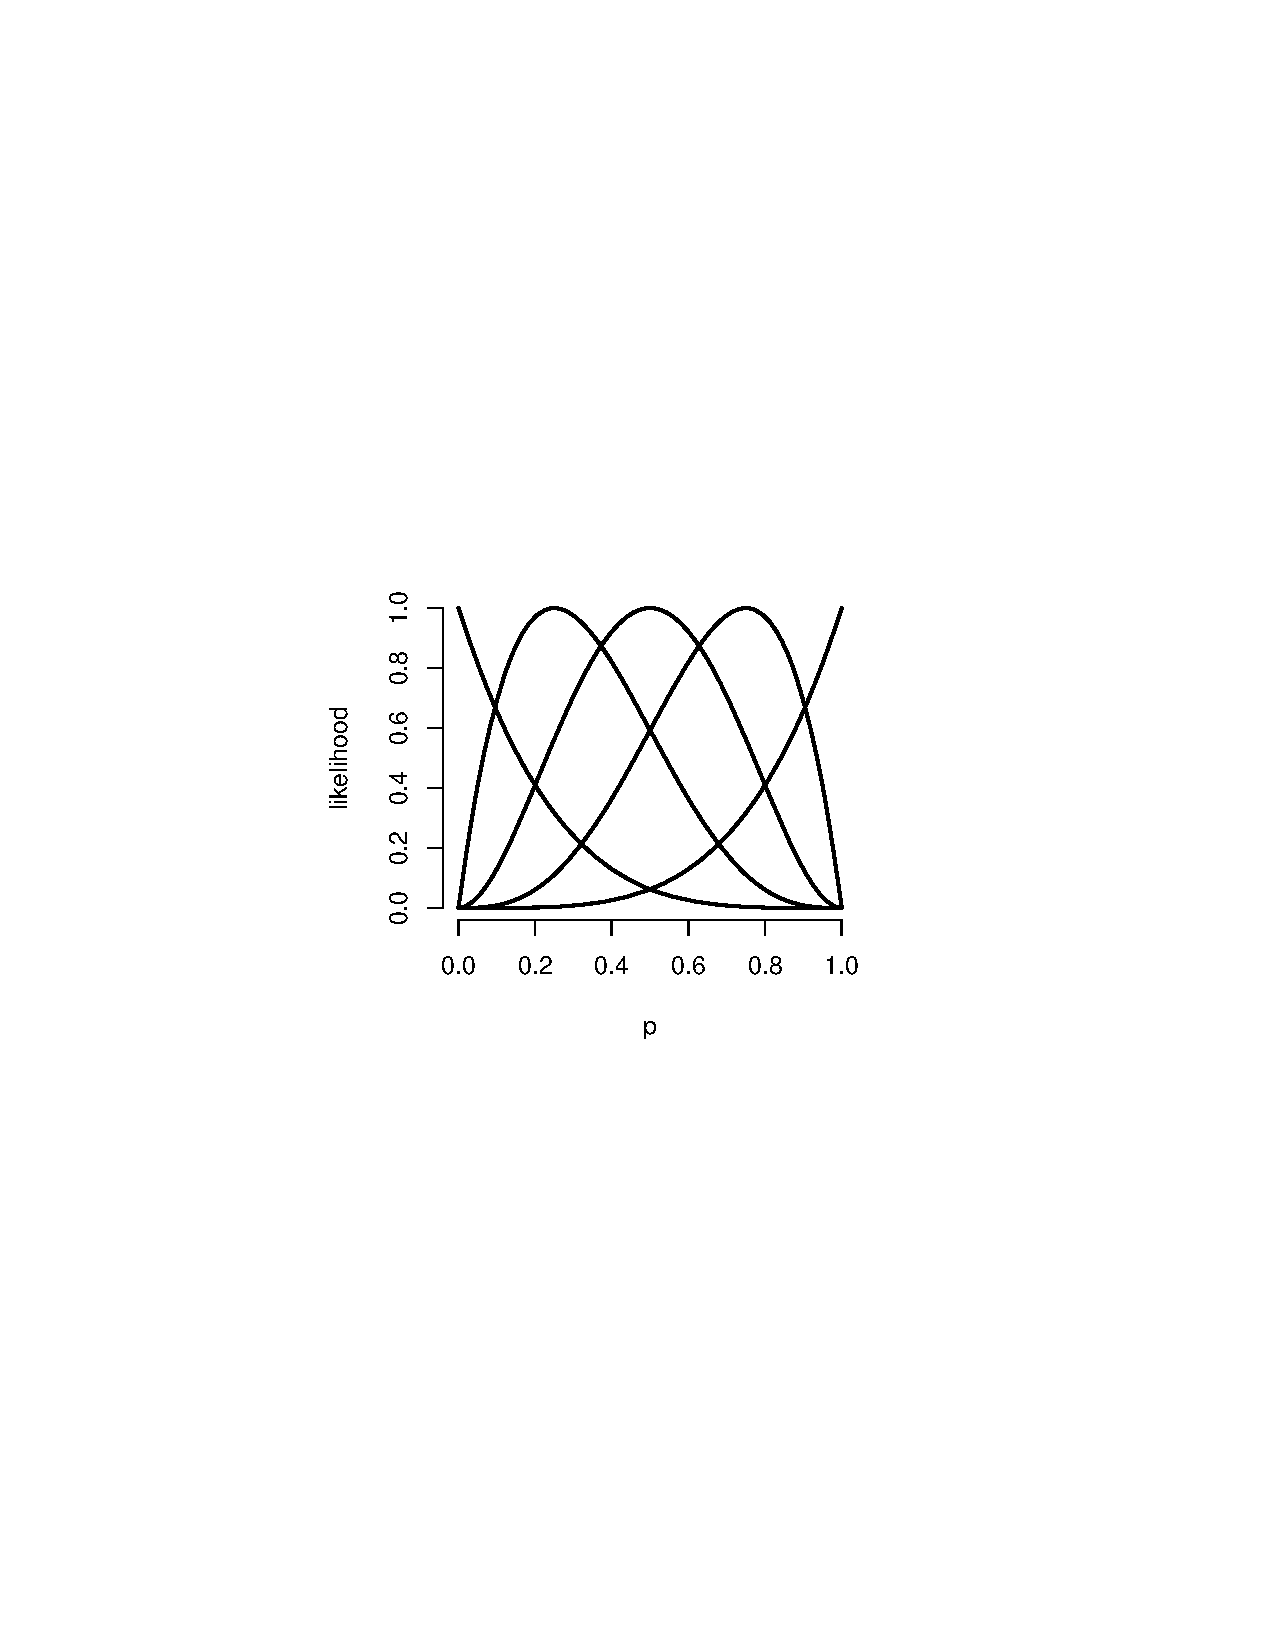
\includegraphics[width=4.5in]{bernoulliLikelihood.pdf}
\end{frame}

\section{Binomial trials}
\begin{frame}\frametitle{Binomial trials}
\begin{itemize}
\item The {\bf binomial random variables} are obtained as the sum of iid Bernoulli trials
\item In specific, let $X_1,\ldots,X_n$ be iid Bernoulli$(p)$; then $X = \sum_{i=1}^n X_i$
  is a binomial random variable
\item The binomial mass function is
$$
P(X = x) = 
\left(
\begin{array}{c}
  n \\ x
\end{array}
\right)
p^x(1 - p)^{n-x}
$$
for $x=0,\ldots,n$
\end{itemize}
\end{frame}

\begin{frame}
\begin{itemize}
\item Recall that the notation 
  $$\left(
    \begin{array}{c}
      n \\ x
    \end{array}
  \right) = \frac{n!}{x!(n-x)!}
  $$ (read ``$n$ choose $x$'') counts the number of ways of selecting $x$ items out of $n$
  without replacement disregarding the order of the items
\item
$$\left(
    \begin{array}{c}
      n \\ 0
    \end{array}
  \right) =
\left(
    \begin{array}{c}
      n \\ n
    \end{array}
  \right) =  1
  $$ 
\end{itemize}
\end{frame}

\begin{frame}\frametitle{Example justification of the binomial likelihood}
\begin{itemize}
\item Consider the probability of getting $6$ heads out of $10$ coin flips from 
  a coin with success probability $p$ 
\item The probability of getting $6$ heads and $4$ tails in any specific
  order is
  $$
  p^6(1-p)^4
  $$
\item There are 
$$\left(
\begin{array}{c}
  10 \\ 6
\end{array}
\right)
$$
possible orders of $6$ heads and $4$ tails
\end{itemize}
\end{frame}

\begin{frame}\frametitle{Example}
\begin{itemize}
\item Suppose a friend has $8$ children, $7$ of which are girls and none are twins
\item If each gender has an independent $50$\% probability for each birth, what's the probability
  of getting $7$ or more girls out of $8$ births?
$$\left(
\begin{array}{c}
  8 \\ 7
\end{array}
\right) .5^{7}(1-.5)^{1}
+
\left(
\begin{array}{c}
  8 \\ 8
\end{array}
\right) .5^{8}(1-.5)^{0} \approx 0.04
$$
\item This calculation is an example of a Pvalue - the probability
  under a null hypothesis of getting a result as extreme or more
  extreme than the one actually obtained
\end{itemize}
\end{frame}

\begin{frame}
  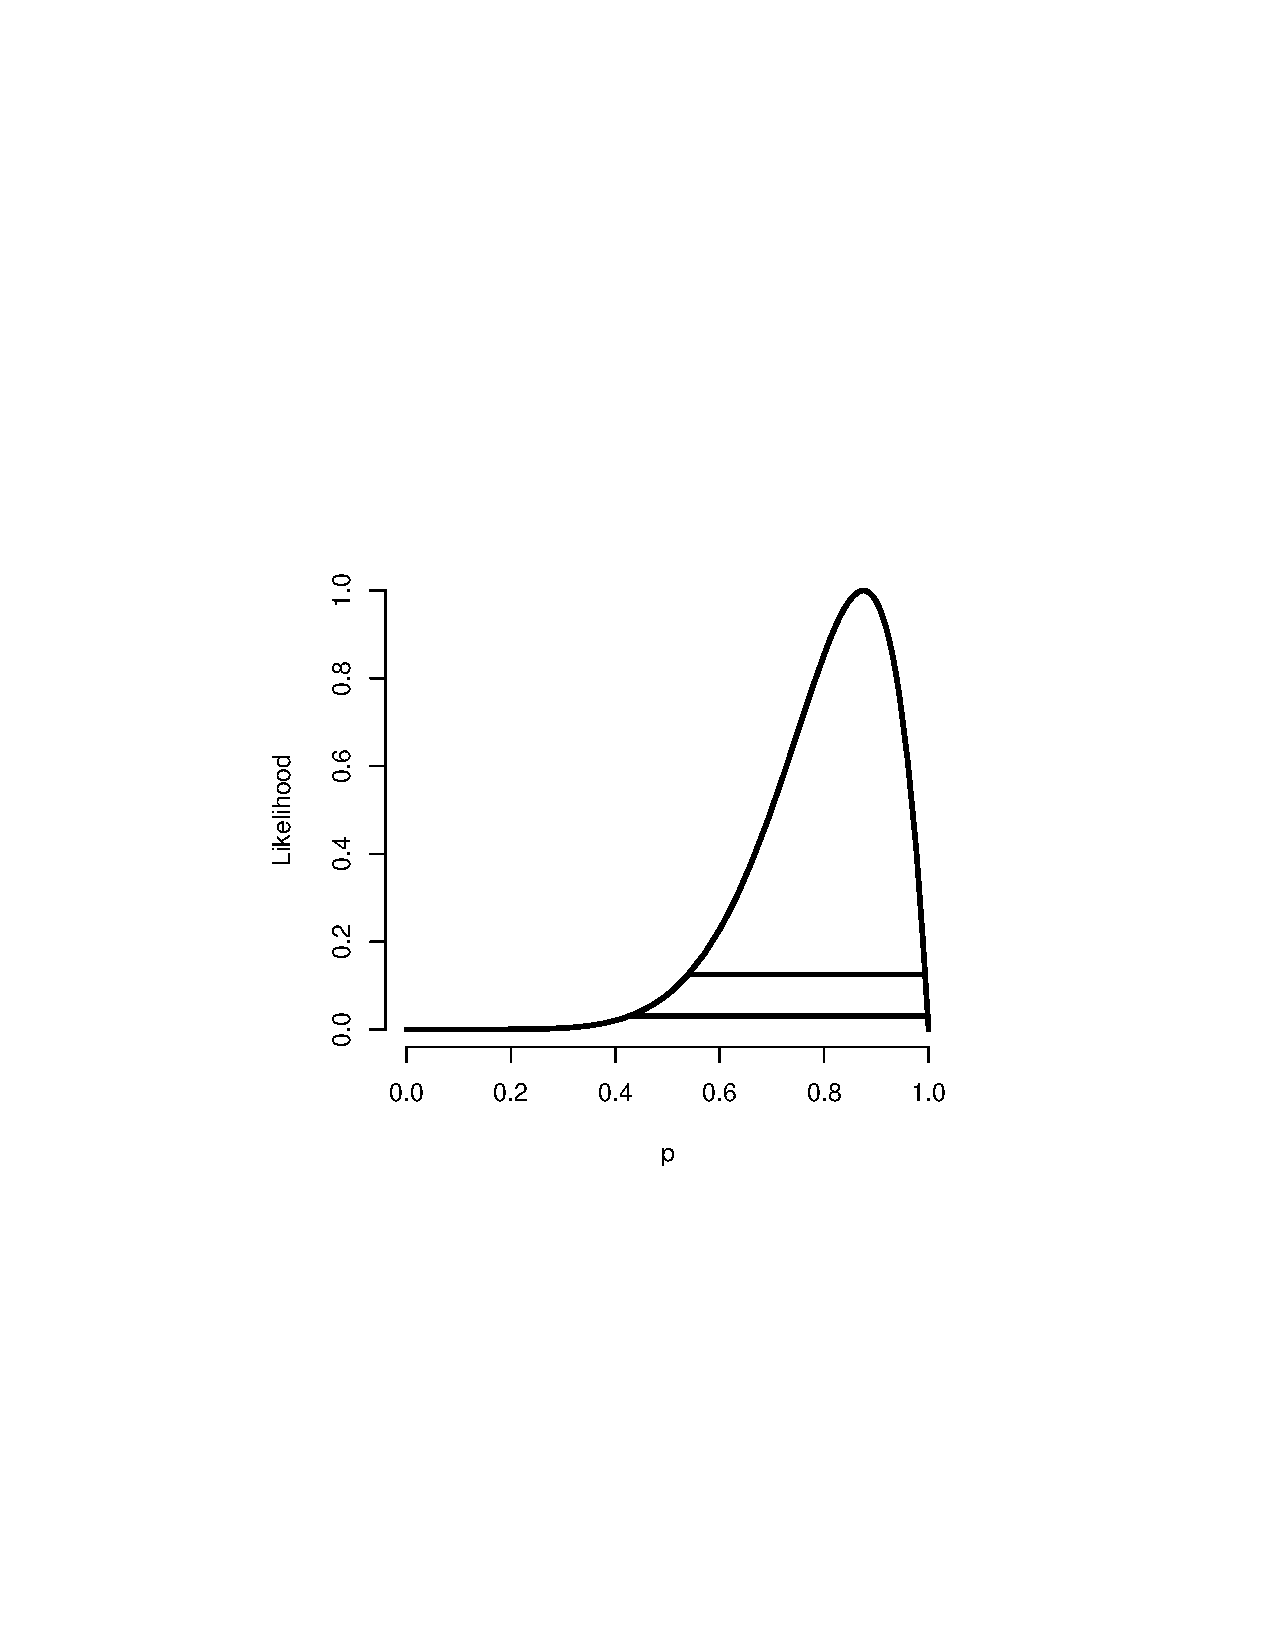
\includegraphics[height=3.5in]{birthLikelihood.pdf}
\end{frame}

\section{The normal distribution}
\begin{frame}\frametitle{The normal distribution}
\begin{itemize}
\item A random variable is said to follow a {\bf normal} or {\bf
    Gaussian} distribution with mean $\mu$ and variance $\sigma^2$ if
  the associated density is
  $$
  (2\pi \sigma^2)^{-1/2}e^{-(x - \mu)^2/2\sigma^2}
  $$
  If $X$ a RV with this density then $E[X] = \mu$ and $\Var(X) = \sigma^2$
\item We write $X\sim \mbox{N}(\mu, \sigma^2)$
\item When $\mu = 0$ and $\sigma = 1$ the resulting distribution is
  called {\bf the standard normal distribution}
\item The standard normal density function is labeled $\phi$
\item Standard normal RVs are often labeled $Z$
\end{itemize}
\end{frame}

\begin{frame}
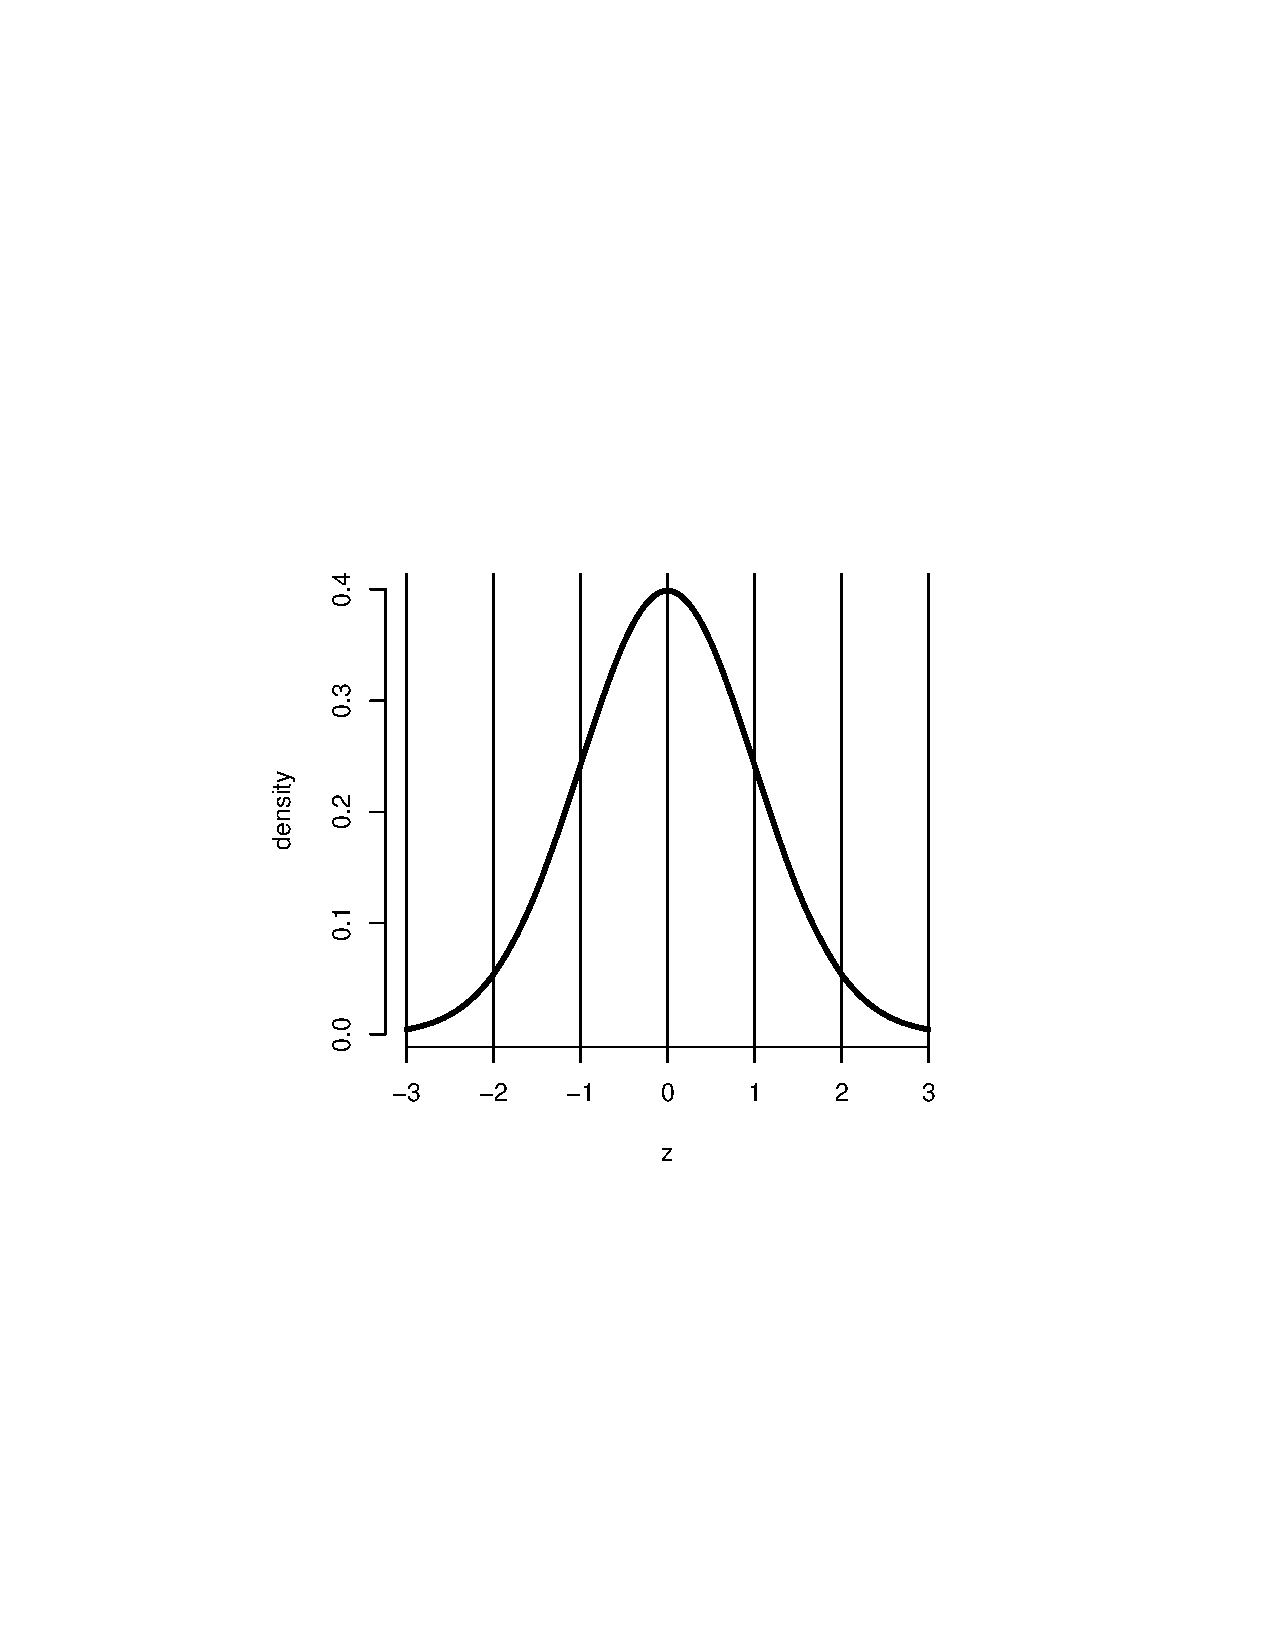
\includegraphics[height=3.5in]{stdNormal.pdf}
\end{frame}

\subsection{Properties}
\begin{frame}\frametitle{Facts about the normal density}
\begin{itemize}
\item If $X \sim \mbox{N}(\mu,\sigma^2)$ the $Z = \frac{X -\mu}{\sigma}$ is standard normal
\item If $Z$ is standard normal $$X = \mu + \sigma Z \sim \mbox{N}(\mu, \sigma^2)$$
\item The non-standard normal density is $$\phi\{(x - \mu) / \sigma\}/\sigma$$
\end{itemize}
\end{frame}

\begin{frame}\frametitle{More facts about the normal density}
  \begin{enumerate}
  \item Approximately $68\%$, $95\%$ and $99\%$  of the normal density lies within
    $1$, $2$ and $3$ standard deviations from the mean, respectively
  \item $-1.28$, $-1.645$, $-1.96$ and $-2.33$ are the $10^{th}$, $5^{th}$, $2.5^{th}$ and $1^{st}$
    percentiles of the standard normal distribution respectively
  \item By symmetry, $1.28$, $1.645$, $1.96$ and $2.33$ are the $90^{th}$,
    $95^{th}$, $97.5^{th}$ and $99^{th}$ percentiles of the standard normal
    distribution respectively
  \end{enumerate}
\end{frame}

\begin{frame}\frametitle{Question}
\begin{itemize}
\item What is the $95^{th}$ percentile of a $N(\mu, \sigma^2)$ distribution?
\item We want the point $x_0$ so that $P(X \leq x_0) = .95$
  \begin{eqnarray*}
    P(X \leq x_0) & = & P\left(\frac{X - \mu}{\sigma} \leq \frac{x_0 - \mu}{\sigma}\right) \\ \\
                  & = & P\left(Z \leq \frac{x_0 - \mu}{\sigma}\right) =  .95
  \end{eqnarray*}
\item Therefore
  $$\frac{x_0 - \mu}{\sigma} = 1.645$$
  or $x_0 = \mu + \sigma 1.645$
\item In general $x_0 = \mu + \sigma z_0$ where $z_0$ is the appropriate standard normal quantile
\end{itemize}
\end{frame}

\begin{frame}\frametitle{Question}
\begin{itemize}
\item What is the probability that a $\mbox{N}(\mu,\sigma^2)$ RV is 2 standard deviations
  above the mean?
\item We want to know
  \begin{eqnarray*}
  P(X > \mu + 2\sigma) & = & 
P\left(\frac{X -\mu}{\sigma} > \frac{\mu + 2\sigma - \mu}{\sigma}\right)    \\ \\
& = & P(Z \geq 2 ) \\ \\ 
& \approx & 2.5\%
  \end{eqnarray*}
\end{itemize}
\end{frame}


\begin{frame}\frametitle{Other properties}
\begin{enumerate}
\item The normal distribution is symmetric and peaked about its mean (therefore
  the mean, median and mode are all equal)
\item A constant times a normally distributed random variable is also
  normally distributed (what is the mean and variance?)
\item Sums of normally distributed random variables are again normally distributed
  even if the variables are dependent (what is the mean and variance?)
\item Sample means of normally distributed random variables are again normally distributed
  (with what mean and variance?)
\item The square of a {\em standard normal} random variable follows what is 
  called {\bf chi-squared} distribution 
\item The exponent of a normally distributed random variables follows what is 
  called the {\bf log-normal} distribution 
\item As we will see later, many random variables, properly
  normalized, {\em limit} to a normal distribution 
\end{enumerate}
\end{frame}

\begin{frame}\frametitle{Question}
If $X_i$ are iid $\mbox{N}(\mu, \sigma^2)$ with a known variance, what is the likelihood for $\mu$?
\begin{eqnarray*}
{\cal L}(\mu) & =    &  \prod_{i=1}^n  (2\pi \sigma^2)^{-1/2}\
exp\left\{-(x_i - \mu)^2/2\sigma^2\right\} \\ \\
              &\propto &  \exp\left\{-\sum_{i=1}^n (x_i - \mu)^2/2\sigma^2\right\} \\ \\
              & =    &  \exp\left\{-\sum_{i=1}^n x_i^2/2\sigma^2 + \mu \sum_{i=1}^n X_i / \sigma^2 - n \mu^2/2\sigma^2\right\}\\
              &\propto & \exp\left\{\mu n \bar x / \sigma^2 - n \mu^2/2\sigma^2\right\}
\end{eqnarray*}
Later we will discuss methods for handling the unknown variance
\end{frame}

\subsection{ML estimate of $\mu$}
\begin{frame}\frametitle{Question}
\begin{itemize}
\item If $X_i$ are iid $\mbox{N}(\mu, \sigma^2)$, with known  variance what's the ML estimate of $\mu$?
\item We calculated the likelihood for $\mu$ on the previous page, the log likelihood is
  $$
  \mu n \bar x / \sigma^2 - n \mu^2/2\sigma^2
  $$
\item The derivative with respect to $\mu$ is 
  $$
  n \bar x / \sigma^2 - n \mu / \sigma ^ 2 = 0
  $$
\item This yields that $\bar x$ is the ml estimate of $\mu$
\item Since this doesn't depend on $\sigma$ it is also the ML estimate with $\sigma$ unknown
\end{itemize}
\end{frame}

\begin{frame}\frametitle{Final thoughts on normal likelihoods}
\begin{itemize}
\item The maximum likelihood estimate for $\sigma^2$ is
  $$
  \frac{\sum_{i=1}^n (X_i - \bar X)^2}{n}
  $$
  Which is the biased version of the sample variance
\item The ML estimate of $\sigma$ is simply the square root of this
  estimate
\item To do likelihood inference, the bivariate likelihood of 
  $(\mu, \sigma)$ is difficult to visualize
\item Later, we will discuss methods for constructing likelihoods for
  one parameter at a time
\end{itemize}
\end{frame}

\end{document}

